\begin{figure}[htbp]
    \centering
    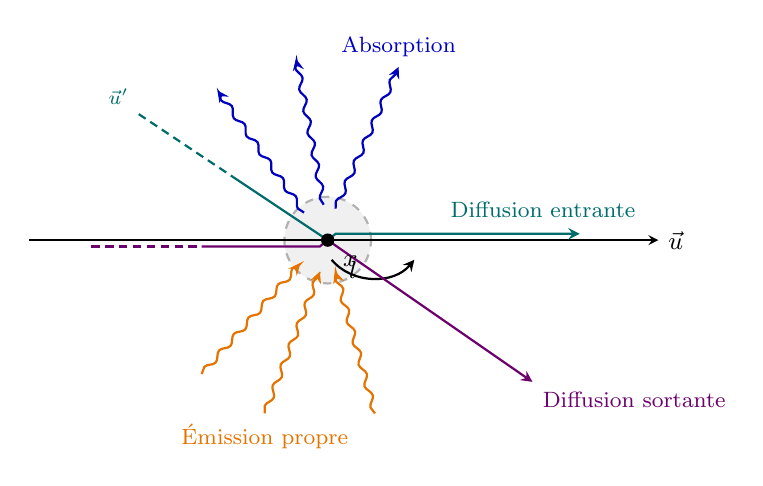
\begin{tikzpicture}[scale=1.0, >=stealth]
        % --- Définition du point central ---
        \coordinate (x) at (0, 0);

        % Cercle de contrôle : remplissage gris léger et contour en pointillés grisés
        \filldraw[fill=gray!12, draw=gray!60, dashed, thick] (x) circle (0.55);

        % --- Axe principal noir u (trait semithick) ---
        \draw[semithick] (-3.8, 0) -- (x);
        \draw[semithick, ->] (x) -- (4.2, 0) node[right, font=\small] {$\vec{u}$};

        % --- Arc de flèche représentant l'avancement dl le long de u ---
        \draw[thick, ->, black] (0.05, -0.25) to[bend right=50] (1.1, -0.25)
            node[at end, below right=4pt, font=\small] {$\dd l$};

        % ==============================================================
        % 1. DIFFUSION ENTRANTE (Vert émeraude / Teal)
        % ==============================================================
        \draw[thick, densely dashed, teal!85!black] (-2.4, 1.6) -- (-1.2, 0.8);
        \draw[thick, teal!85!black] (-1.2, 0.8) -- (x);
        \draw[thick, ->, teal!85!black] (x) -- (0.1, 0.08) -- (3.2, 0.08)
            node[pos=0.85, above=2pt, font=\footnotesize] {Diffusion entrante};
        \node[teal!85!black, font=\scriptsize, above left] at (-2.4, 1.6) {$\vec{u}'$};

        % ==============================================================
        % 2. DIFFUSION SORTANTE (Violet)
        % ==============================================================
        \draw[thick, densely dashed, violet!85!black] (-3.0, -0.08) -- (-1.6, -0.08);
        \draw[thick, violet!85!black] (-1.6, -0.08) -- (-0.1, -0.08) -- (x);
        \draw[thick, ->, violet!85!black] (x) -- (2.6, -1.8)
            node[below right, font=\footnotesize] {Diffusion sortante};

        % ==============================================================
        % 3. ABSORPTION (Bleu cobalt : flèches ondulées quittant x)
        % ==============================================================
        \draw[thick, ->, blue!75!black, decorate, decoration={snake, amplitude=1pt, segment length=8pt}] 
            (0.1, 0.4) -- (0.9, 2.2)
            node[above, font=\footnotesize] {Absorption};
        \draw[thick, ->, blue!75!black, decorate, decoration={snake, amplitude=1pt, segment length=8pt}] 
            (-0.3, 0.35) -- (-1.4, 1.9);
        \draw[thick, ->, blue!75!black, decorate, decoration={snake, amplitude=1pt, segment length=8pt}] 
            (-0.05, 0.45) -- (-0.4, 2.3);

        % ==============================================================
        % 4. ÉMISSION PROPRE (Orange cuivré : flèches ondulées convergeant vers x)
        % ==============================================================
        \draw[thick, ->, orange!90!black, decorate, decoration={snake, amplitude=1pt, segment length=8pt}] 
            (-0.8, -2.2) -- (-0.1, -0.4)
            node[below, at start, font=\footnotesize] {Émission propre};
        \draw[thick, ->, orange!90!black, decorate, decoration={snake, amplitude=1pt, segment length=8pt}] 
            (0.6, -2.2) -- (0.1, -0.4);
        \draw[thick, ->, orange!90!black, decorate, decoration={snake, amplitude=1pt, segment length=8pt}] 
            (-1.6, -1.7) -- (-0.35, -0.3);

        % Point central rempli de noir plein par-dessus les tracés
        \filldraw[fill=black, draw=black] (x) circle (2.2pt) 
            node[below right=2pt, font=\small] {$x$};
    \end{tikzpicture}
    \caption{Bilan des interactions locales de l'ETR en un point matériel $x$ sur l'élément de longueur $\dd l$ le long de la direction $\vec{u}$.}
    \label{fig:etr_bilan_interactions_simple}
\end{figure}